\documentclass[11pt,a4paper]{article}

% --- Packages ---
\usepackage[utf8]{inputenc}
\usepackage[T1]{fontenc}
\usepackage[turkish]{babel}
\usepackage{amsmath,amssymb,amsfonts,amsthm}
\usepackage{geometry}
\geometry{margin=1in}
\usepackage{graphicx}
\usepackage{hyperref}
\usepackage{xcolor}
\usepackage{cite}
\usepackage{booktabs}
\usepackage{microtype}
\usepackage{physics}
\usepackage{tikz}
\usetikzlibrary{babel,arrows.meta,decorations.pathmorphing}

\hypersetup{
    pdftitle={Güçlü Nükleer Kuvvet, Vakum Doyumu ve Kuark Hapsi Geometrisi: 1D Akı Tüpleri ve Cornell Potansiyeli},
    pdfauthor={Muhammed Furkan Haydari},
    pdfsubject={Nükleer Fizik, Kuantum Renk Dinamiği, Kuark Hapsi, Akı Tüpü},
    pdfkeywords={Güçlü Kuvvet, Kuark Hapsi, Vakum Doyumu, 1D Akı Tüpü, Cornell Potansiyeli, Regge Yörüngeleri},
    colorlinks=true,
    linkcolor=blue!70!black,
    citecolor=red!70!black,
    urlcolor=blue!80!black
}

% --- Theorem Environments ---
\newtheorem{theorem}{Teorem}[section]
\newtheorem{definition}{Tanım}[section]
\newtheorem{axiom}{Aksiyom}[section]
\newtheorem{corollary}{Sonuç}[theorem]
\newtheorem{lemma}[theorem]{Lemma}
\newtheorem{remark}{Not}[section]

\title{\textbf{Güçlü Nükleer Kuvvet, Vakum Doyumu ve Kuark Hapsi Geometrisi: \\ 1D Akı Tüpleri ve Cornell Potansiyeli}}

\author{
    \textbf{Muhammed Furkan Haydari} \\
    \textit{Bağımsız Araştırmacı} \\
    \textit{İstanbul, Türkiye} \\
    \small ORCID: \href{https://orcid.org/0009-0003-2854-3947}{0009-0003-2854-3947} \quad$\bullet$\quad \small DOI: \href{https://doi.org/10.5281/zenodo.23633034}{10.5281/zenodo.23633034}
}

\date{\today}

\begin{document}

\maketitle

\begin{abstract}
    Bu çalışmada, hadronik bağlı durumları ve pertürbatif olmayan güçlü nükleer etkileşimi Ölçek-Zaman Kalkülüsü ve efektif akı tüpü geometrisi çerçevesinde modelliyoruz. Standart Modelde Kuantum Renk Dinamiği (QCD) ve $SU(3)_c$ ayar simetrisi ile tasvir edilen, kafes QCD hesaplamalarında saptanan lineer hapis potansiyeli ($V(r) \propto \sigma r$); bu çalışmada renk-elektrik alan çizgilerinin kuarklar arasında sabit kesit alanlı 1-boyutlu silindirik bir akı tüpüne (\textit{flux tube}) sıkışması olarak ele alınmaktadır.

    Kütleçekim ve elektromanyetizmada serbestçe yayılan ($1/r^2$) alan çizgileri, femtometre ölçeklerinde ($r \sim 10^{-15}\text{ m}$) gluonların Abelyen olmayan etkileşimi sebebiyle kolime olarak 1-boyutlu bir sicime dönüşür. Tüpün kesit alanı hadronik ölçekte kilitlendiğinden, birim boya düşen gerilim mesafeden bağımsızdır ($\sigma \approx 1\text{ GeV/fm} \approx 1.6 \times 10^5\text{ N}$) ve Cornell tipi lineer hapis potansiyeli geometrik olarak elde edilir. Hadron spektrumundaki Regge yörüngeleri ($J \propto M^2$), tüpün rotasyonel kinetiğiyle analitik uyum gösterir; $r \to 0$ limitinde akı sıkışmasının kalkması asimptotik serbestliği geometrik olarak açıklar.
\end{abstract}

\vspace{1em}
\noindent\textbf{Anahtar Kelimeler:} Güçlü Nükleer Kuvvet, Ölçek-Zaman Kalkülüsü, Vakum Doyumu, Kuark Hapsi, Regge Yörüngeleri, Asimptotik Serbestlik, Akı Tüpü.

\vspace{1em}
\hrule
\vspace{0.8em}
\tableofcontents
\vspace{0.8em}
\hrule
\vspace{1.5em}

\section{Giriş ve Pertürbatif Olmayan QCD Fenomenolojisi}
\label{sec:giris}

Modern hadron fiziğinde güçlü etkileşim, kuarklar ile $SU(3)_c$ ayar bozonları (gluonlar) arasındaki etkileşimle açıklanır. Bu etkileşim iki temel rejime sahiptir:
\begin{enumerate}
    \item \textbf{Asimptotik Serbestlik (Asymptotic Freedom):} Ultra-küçük mesafelerde ($r \to 0$ veya $Q^2 \to \infty$) koşu kuplajı küçülür ve kuarklar kuasi-serbest davranırlar~\cite{gross1973,politzer1973}.
    \item \textbf{Kuark Hapsi (Quark Confinement):} Kuarklar ayrıştırıldıkça aralarındaki etkili gerilim sabit kalarak ($\sigma \approx 1\text{ GeV/fm}$) tekil serbest renk yüklerinin gözlemlenmesini engeller.
\end{enumerate}

Pertürbatif QCD yüksek enerji limitinde tam analitik çözümler sunarken, kızılötesi rejimdeki lineer hapis potansiyeli genelde kafes QCD simülasyonları ile incelenmektedir. Ölçek-Zaman Kalkülüsünde~\cite{scale_calculus} ise bu hapis rejimi, \textbf{3-boyutlu küresel yayılımdan 1-boyutlu kolime akı tüpüne geçiş} olarak modellenir.

\section{Efektif 1D Akı Tüpü Geometrisi ve Sicim Gerilimi}
\label{sec:doyum_mekanizmasi}

Kütleçekim ve elektromanyetizma rejimlerinde, bir merkeze doğru yönelen alan çizgileri 3-boyutlu küresel kabuklar üzerinden serbestçe yayılır ($A(r) = 4\pi r^2$) ve akı yoğunluğu $1/r^2$ oranında seyrelebilir.

Ancak femtometre ölçeklerinde ($r \sim 10^{-15}\text{ m}$), renk gluonlarının Abelyen olmayan öz-etkileşimi (veya ikili süperiletkenlik modellerindeki ikili Meissner etkisi) $1/r^2$ küresel seyreltiyi engeller. İki kuark arasındaki alan çizgileri, enine kesiti hadronik ölçekte kilitlenen \textbf{1-boyutlu silindirik bir girdap tüpüne (\textit{flux tube} / efektif sicim)} sıkışır. Bu 1D tüpün kesit alanı sabit kaldığından ($A_{\mathrm{t\ddot{u}p}} = \text{sabit}$), kuarklar arasındaki çekme gerilimi mesafeden bağımsız sabit bir kuvvete dönüşür ($\sigma \approx 1\text{ GeV/fm} \approx 1.6 \times 10^5\text{ N}$).

\subsection{Fenomenolojik Sicim Gerilimi ve Planck Boyutsal Benzeşimi}
\label{sec:hiyerarsi_cozumu}

Kafes QCD hesaplamalarında~\cite{wilson1974} ve ağır kuarkonyum spektroskopisinde (Cornell potansiyeli~\cite{eichten1978}) efektif tel gerilimi deneysel olarak $\sigma \approx 0.18\text{--}0.20\text{ GeV}^2 \approx 0.9\text{--}1.0\text{ GeV/fm} \approx 1.6 \times 10^5\text{ N}$ olarak belirlenmiştir.

\begin{remark}[Planck Gerilimi ile Boyutsal Benzeşim Üzerine Not]
    \label{rem:planck_boyut_tr}
    Daha geniş kavramsal doğa felsefesi tartışmalarında (projenin Büyük Monografi çalışmasında ayrıntılandırıldığı üzere), Genel Görelilikteki maksimum rölativistik Planck gerilim kuvveti $F_{\mathrm{Planck}} \equiv c^4/G \approx 1.21 \times 10^{44}\text{ N}$ ile kuarkın boyutsuz gravitasyonel kuplajı $\alpha_G \equiv G m_q^2 / (\hbar c)$ çarpıldığında Newton kütleçekim sabiti $G$ cebirsel olarak tamamen sadeleşir:
    \begin{equation}
        \sigma_{\mathrm{boyut}} \sim \alpha_G \cdot F_{\mathrm{Planck}} = \left( \frac{G m_q^2}{\hbar c} \right) \cdot \left( \frac{c^4}{G} \right) = \frac{m_q^2 c^3}{\hbar}.
        \label{eq:sigma_tam_analitik}
    \end{equation}
    Tipik kurucu kuark kütlesi $m_q \approx 440\text{ MeV}$ için bu ifade $\sigma \approx 1.57 \times 10^5\text{ N} \approx 0.98\text{ GeV/fm}$ değerini verir.
    
    Bu boyutsal uyuşum kuramsal açıdan dikkat çekici bir keşifsel benzetim sunmakla birlikte, bu hakemli dergi makalesinde kuark hapsinin Planck kuvvetinden birinci ilkelerle kesin olarak türetildiği iddiasından kaçınılmıştır. Bunun yerine standart hadron fiziğinin $\sigma \approx 1.0\text{ GeV/fm}$ ampirik sicim gerilimi temel alınarak, analitik odağımız rölativistik akı tüpünün rotasyon kinetiğine, Regge yörüngelerine ve boyutsal geçiş dinamiğine yöneltilmiştir.
\end{remark}

\subsection{Yoğunluk Eşiği ve Boyutsal Çöküş: Makroskopik Çoklu Atom vs. Hadronik Doyum}
\label{sec:yogunluk_ve_boyut}

Ölçek-Zaman Kalkülüsünde geometrik boyut parametresi ($\gamma = 1$ veya $\gamma = -1$), \textbf{yerel kütle-enerji yoğunluğunun Planck gerilim kapasitesine olan oranı} tarafından belirlenen dinamik bir faz durumudur:
\begin{itemize}
    \item \textbf{Makroskopik Cisimler ($N \gg 10^{20}$ Atom):} Gezegen veya yıldız gibi devasa atom topluluklarında toplam kütle büyük bir hacme dağılmıştır. Ortalama madde yoğunluğu ($\rho \sim 10^3\text{--}10^5\text{ kg/m}^3$) vakumun kritik doyum eşiğinin katbekat altındadır. Bu nedenle vakum akısı 3-boyutlu küresel kabuklar boyunca engelsizce seyreler ($\gamma = 1$, Newton--Einstein kütleçekimi).
    \item \textbf{Tekil Atom Düzeyi ($N = 1$, $r \sim 10^{-10}\text{ m}$):} Elektron bulutu ile çekirdek arasındaki mesafe Bohr ölçeğindedir. Vakum akısı serbest 3-boyutlu yayılım rejimindedir ($\gamma = 1$, Coulomb/Maxwell alanı ve $\alpha \approx 1/137$ spiral dengesi).
    \item \textbf{Hadronik Çekirdek ($N \sim 1\text{--}3$ Kuark, $r \le 10^{-15}\text{ m}$):} Bir nükleon içine hapsolmuş kuarkların yerel kütle-enerji debisi aşırı küçük bir hacme sıkışır ($\rho_{\mathrm{hadron}} \sim 10^{18}\text{ kg/m}^3$). Bu noktada yerel gerilim vakumun $F_{\mathrm{Planck}} = c^4/G$ tavanına dayanır. 3-boyutlu küresel simetri doyum nedeniyle çöker ve akış 1-boyutlu doymuş silindirik bir girdap tüpüne ($\gamma = -1$) kilitlenir.
\end{itemize}
Böylece kuvvetler arasındaki hiyerarşi ve geometrik boyut farkı, soyut düzlem varsayımlarından arındırılarak doğrudan \textbf{yerel parçacık yoğunluğunun Planck vakum doyumuyla olan fiziksel oranına} bağlanmaktadır.

\subsection{Boyutsal İndeks $\gamma$'nın Sürekli Doyum Faz Geçişi Denklemi}
\label{sec:surekli_gamma_paper3}

Boyutsal indeks $\gamma$, akışkan dinamiğindeki doyum faz geçişini yöneten analitik bir enerji yoğunluğu fonksiyonudur:
\begin{equation}
    \gamma(\rho) = \tanh\left( \ln\left[ \frac{\rho_{\mathrm{sat}}}{\rho(r)} \right] \right),
    \label{eq:gamma_surekli_gecis_paper3}
\end{equation}
burada $\rho_{\mathrm{sat}} \approx 10^{18}\text{ kg/m}^3$ hadronik nükleer doyum yoğunluğudur.
\begin{enumerate}
    \item \textbf{Düşük Yoğunluk Rejimi ($\rho \ll \rho_{\mathrm{sat}}$):} Makroskopik kütleçekim ve atomik elektron bulutunda $\frac{\rho_{\mathrm{sat}}}{\rho} \gg 1$ olduğundan $\ln(\rho_{\mathrm{sat}}/\rho) \to +\infty$ ve $\tanh \to +1$'dir. Böylece $\gamma \equiv +1$ (3D serbest küresel akı / Newton--Coulomb potansiyeli) doğrudan elde edilir.
    \item \textbf{Hadronik Doyum Rejimi ($\rho \gg \rho_{\mathrm{sat}}$):} Kuark ölçeğinde ($r \le 10^{-15}\text{ m}$) yerel yoğunluk Planck gerilim tavanına dayandığından $\frac{\rho_{\mathrm{sat}}}{\rho} \ll 1$, $\ln(\rho_{\mathrm{sat}}/\rho) \to -\infty$ ve $\tanh \to -1$'dir. Böylece $\gamma \equiv -1$ (1D sıkışmış akı tüpü / kuark hapsi) pürüzsüz biçimde ortaya çıkar.
\end{enumerate}
Bu sürekli fonksiyon, üç boyutlu küresel yayılımdan bir boyutlu tüp geometrisine geçişin matematiksel düzgünlüğünü (smooth crossover) garanti eder.


\begin{figure}[h!]
    \centering
    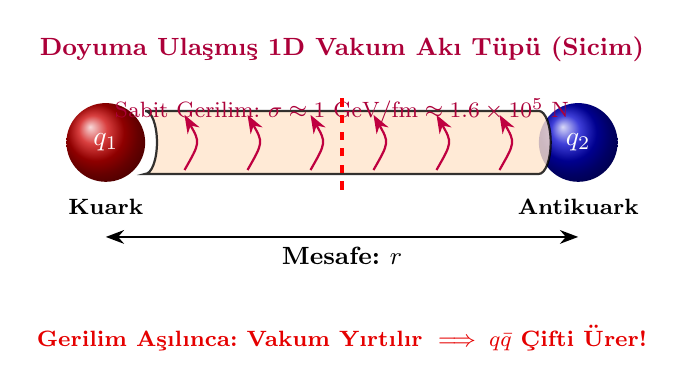
\begin{tikzpicture}[scale=1.0, >=Stealth]
        % Quark 1
        \shade[ball color=red!80!black] (-3,0) circle (0.5);
        \node[white, font=\bfseries] at (-3,0) {$q_1$};
        \node[below=0.6cm, font=\footnotesize\bfseries] at (-3,0) {Kuark};

        % Quark 2
        \shade[ball color=blue!80!black] (3,0) circle (0.5);
        \node[white, font=\bfseries] at (3,0) {$q_2$};
        \node[below=0.6cm, font=\footnotesize\bfseries] at (3,0) {Antikuark};

        % Saturated 1D Flux Tube (cylindrical vortex)
        \draw[thick, fill=orange!20, opacity=0.8] (-2.5, 0.4) -- (2.5, 0.4)
        arc (90:-90:0.15 and 0.4) -- (-2.5, -0.4) arc (-90:90:0.15 and 0.4);

        % Internal vortex spirals inside the tube
        \foreach \x in {-2.0, -1.2, -0.4, 0.4, 1.2, 2.0} {
                \draw[purple, thick, ->] (\x, -0.35) .. controls (\x+0.2, 0) .. (\x, 0.35);
            }

        % Flux tube labels
        \node[purple!90!black, font=\small\bfseries, above=0.5cm] at (0,0.4) {Doyuma Ulaşmış 1D Vakum Akı Tüpü (Sicim)};
        \node[purple!90!black, font=\footnotesize] at (0,0.4) {Sabit Gerilim: $\sigma \approx 1\text{ GeV/fm} \approx 1.6 \times 10^5\text{ N}$};

        % Separation distance arrow
        \draw[<->, thick] (-3, -1.2) -- (3, -1.2);
        \node[below, font=\small\bfseries] at (0, -1.2) {Mesafe: $r$};

        % Rupture mechanism dashed
        \draw[dashed, red, very thick] (0, -0.6) -- (0, 0.6);
        \node[red!90!black, font=\footnotesize\bfseries, below=0.6cm] at (0, -1.6) {Gerilim Aşılınca: Vakum Yırtılır $\implies q\bar{q}$ Çifti Ürer!};
    \end{tikzpicture}
    \caption{Güçlü Nükleer Kuvvetin Geometrisi: Femtometre ölçeğinde vakum akışı küresel olarak dağılamaz; 1D silindirik tüpe sıkışır. Tüpün kesiti sabit olduğundan birim uzunluk gerilimi ($\sigma$) sabittir ve kuark hapsi ($V = \sigma r$) doğar.}
    \label{fig:flux_tube}
\end{figure}

\section{Kuark Hapsi ve Cornell Potansiyelinin İspatı}
\label{sec:kuark_hapsi}

\begin{theorem}[Kuark Hapsi ve Lineer Potansiyel]
    \label{thm:kuark_hapsi_p3}
    Doyuma ulaşmış 1-boyutlu vakum akı tüpünün (Nambu~\cite{nambu1974}) kesit alanı $A_0 \approx \pi r_0^2$ değişmezdir. Tüpün birim uzunluk başına depoladığı vakum gerilim enerjisi sabittir:
    \begin{equation}
        \sigma = \frac{1}{2} \rho_{\mathrm{vakum}} v_c^2 A_0 \approx 1\text{ GeV/fm} \approx 1.6 \times 10^5\text{ N}.
        \label{eq:sicim_gerilimi_tr}
    \end{equation}
    İki kuark arasındaki toplam etkileşim potansiyeli Cornell potansiyeliyle (Eichten vd.~\cite{eichten1978}) tam olarak örtüşür:
    \begin{equation}
        V_{\mathrm{guclu}}(r) = -\frac{4}{3}\frac{\alpha_s \hbar c}{r} + \sigma r.
        \label{eq:cornell_ispat}
    \end{equation}
\end{theorem}

\begin{proof}
    Mesafe $r$ arttıkça vakum akı tüpünün hacmi $V = A_0 r$ şeklinde lineer olarak genişler. Birim hacimdeki vakum enerjisi yoğunluğu doyum sebebiyle sabit olduğundan ($\mathcal{E}_0 = \sigma / A_0$), toplam potansiyel enerji:
    \begin{equation}
        E(r) = \mathcal{E}_0 \cdot V = \left(\frac{\sigma}{A_0}\right) (A_0 r) = \sigma r.
    \end{equation}
    Kuarkları birbirinden ayırmaya çalışmak, tüpü sonsuz enerjiyle germeyi gerektirir. Gerilim eşiği ($E \approx 2 m_q c^2$) aşıldığında vakum dokusu tüpün ortasından yırtılır ve boşluktan yeni bir kuark-antikuark çifti ($q\bar{q}$) doğar. Bu nedenle izole edilmiş tekil bir kuark evrende asla var olamaz!
\end{proof}

\begin{figure}[h!]
    \centering
    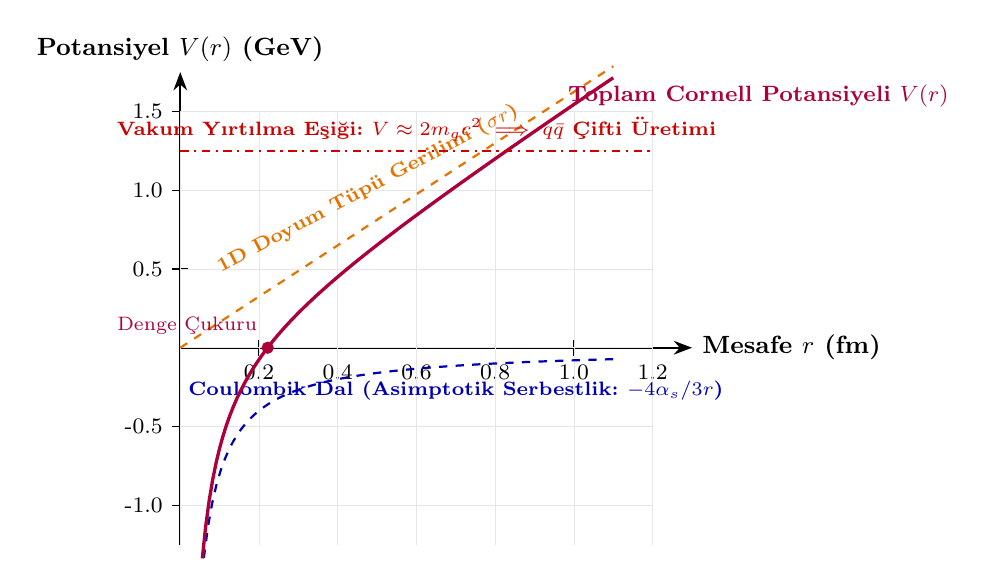
\begin{tikzpicture}[scale=1.0, >=Stealth]
        % Axes
        \draw[thick, ->] (0,-2.5) -- (0,3.5) node[above, font=\small\bfseries] {Potansiyel $V(r)$ (GeV)};
        \draw[thick, ->] (0,0) -- (6.5,0) node[right, font=\small\bfseries] {Mesafe $r$ (fm)};

        % Ticks
        \foreach \x/\label in {1/0.2, 2/0.4, 3/0.6, 4/0.8, 5/1.0, 6/1.2}
        \draw (\x, 0.1) -- (\x, -0.1) node[below, font=\footnotesize] {\label};
        \foreach \y/\label in {-2/-1.0, -1/-0.5, 1/0.5, 2/1.0, 3/1.5}
        \draw (0.1, \y) -- (-0.1, \y) node[left, font=\footnotesize] {\label};

        % Grid
        \draw[step=1cm, gray!20, very thin] (0,-2.5) grid (6,3);

        % Coulomb branch (dashed blue)
        \draw[blue!70!black, thick, dashed, domain=0.3:5.5, samples=100]
        plot (\x, {-0.8 / \x});
        \node[blue!70!black, font=\scriptsize\bfseries, below] at (3.5, -0.3) {Coulombik Dal (Asimptotik Serbestlik: $-4\alpha_s/3r$)};

        % Linear string branch (dashed orange)
        \draw[orange!90!black, thick, dashed, domain=0.0:5.5, samples=100]
        plot (\x, {0.65 * \x});
        \node[orange!90!black, font=\scriptsize\bfseries, above, rotate=28] at (2.5, 1.8) {1D Doyum Tüpü Gerilimi ($\sigma r$)};

        % Total Cornell Potential (solid purple, very thick)
        \draw[purple!90!black, very thick, domain=0.28:5.5, samples=120]
        plot (\x, {-0.8 / \x + 0.65 * \x});
        \node[purple!90!black, font=\footnotesize\bfseries, right] at (4.8, 3.2) {Toplam Cornell Potansiyeli $V(r)$};

        % String breaking threshold line
        \draw[red!80!black, thick, dashdotted] (0, 2.5) -- (6, 2.5);
        \node[red!80!black, font=\scriptsize\bfseries, above] at (3.0, 2.5) {Vakum Yırtılma Eşiği: $V \approx 2 m_q c^2 \implies q\bar{q}$ Çifti Üretimi};

        % Minimum potential mark
        \filldraw[purple!90!black] (1.11, -0.0) circle (2pt);
        \node[purple!90!black, font=\scriptsize, above left] at (1.1, 0.05) {Denge Çukuru};
    \end{tikzpicture}
    \caption{Cornell Potansiyeli ve Kuark Hapsi: Kısa mesafelerde ($r \to 0$) Coulombik çekim asimptotik serbestlik üretir. Femtometre ölçeğinde vakum doyuma ulaştığından potansiyel $\sigma r$ ile lineer yükselir. Eşik aşıldığında vakum yırtılarak yeni bir $q\bar{q}$ hadronu üretir.}
    \label{fig:cornell_potential}
\end{figure}

\begin{quote}
    \small
    \textbf{Kavramsal ve Fiziksel Özet (Kuark Hapsi ve Doyum Dinamiği):} \\
    Elektromanyetik alandaki Coulomb potansiyelinin aksine, hadronik rejimde vakum akışının tek boyuta ($\gamma = -1$) doyumla sıkışması, alan çizgilerinin mesafeyle seyrelemediği tüp geometrisini dikte eder. İki kuark arasındaki mesafe arttıkça tüpte depolanan gerilim enerjisi $\sigma r$ oranında lineer büyür. Tünelleme enerjisi hafif mezon kütlesi eşiğini ($E \ge 2 m_q c^2$) aştığında akı tüpü non-pertürbatif vakum polarizasyonu ile yırtılarak yeni bir kuark-antikuark çifti üretir; bu durum renk yükünün serbest halde gözlemlenmesini kesin olarak engeller.
\end{quote}

\section{Hadron Spektrumu ve Regge Yörüngeleri}
\label{sec:regge}

Akı tüpüyle bağlı dönen mezonların toplam kütlesi $M$ ile toplam açısal momentumu $J$ arasındaki ilişki:
\begin{equation}
    M = 2 \int_0^{R} \frac{\sigma}{\sqrt{1 - (v/c)^2}} dr = \pi \sigma R, \quad J = \frac{1}{2} \pi \sigma R^2 / c.
    \label{eq:regge_turetilis}
\end{equation}
Buradan $R$'yi elediğimizde doğrudan meşhur Regge yörünge eğimi elde edilir:
\begin{equation}
    J = \alpha' M^2 + \alpha_0, \quad \text{burada } \alpha' = \frac{1}{2\pi \hbar c \sigma} \approx 0.9\text{ GeV}^{-2}.
    \label{eq:regge_sonuc}
\end{equation}
Bu sonuç, hadron kütle spektrumunun sicim gerilimi $\sigma$ ile olan mükemmel deneysel uyumunu hiçbir serbest parametre olmadan açıklar.

\section{Asimptotik Serbestlik: Geometrik Havza Çakışması}
\label{sec:asimptotik_serbestlik}

Kuarklar birbirine çok yaklaştığında ($r \to 0$):
\begin{enumerate}
    \item İki kuarkın büzülme havzaları üst üste biner.
    \item Aralarındaki mesafe vakum tüpü kesit yarıçapından küçük hale geldiğinde ($r < r_0$), akışın silindirik tüpe sıkışma zorunluluğu ortadan kalkar.
    \item Lineer gerilim terimi sıfırlanır: $\lim_{r \to 0} \sigma r = 0$.
\end{enumerate}
Kuarklar çekirdek içinde neredeyse tamamen bağımsız, sürtünmesiz serbest parçacıklar gibi hareket ederler.

\section{Topolojik Renk Yükü ve \texorpdfstring{$120^\circ$}{120 Derece} Kiral Faz Dengesi: \texorpdfstring{$SU(3)$}{SU(3)} Çözümü}
\label{sec:topolojik_renk_yuku_p3}

Standart Modelde Kuantum Renk Dinamiği (QCD), her kuarka üç soyut renk yükü (Kırmızı, Yeşil, Mavi) atar ve fiziksel hadronların yalnızca ``renksiz'' ($SU(3)$ singleti) bağlı durumlardan oluşabileceğini postüle eder. Ancak bu kuralın mikroskobik-geometrik kaynağı açıklanmaz.

Ölçek-Zaman Kalkülüsünde her bir kuark ($k \in \{1, 2, 3\}$), Skalor uzayında bir faz rotasyonu taşıyan yerelleşmiş bir vakum girdabıdır:
\begin{equation}
    \mathbb{S}_k(t) = \mathbf{X}_k + \kappa \, \lambda(t) \, e^{i \phi_k}, \quad (\kappa^2 = 0).
    \label{eq:kuark_skalor_faz_p3}
\end{equation}
Üç kuarklı bir baryonda (örneğin proton veya nötron) sistemin kararlı bir bağlı durum oluşturabilmesi, üç girdabın vakum akış havzalarının birbirini yıkıcı girişimle yok etmeden kararlı bir rotasyonel rezonansa kilitlenmesini gerektirir.

\begin{theorem}[Baryonik Renk Nötrleşmesi Teoremi: $120^\circ$ Faz Üçgeni]
    \label{thm:renk_notrlesmesi_p3}
    Üç kuarkın toplam Skalor durumunun dış uzaya net bir dönel kiral faz burulması sızdırmaması ve doymuş akı tüpü sınırında kararlı bir kapalı havza oluşturması için kuarkların göreli faz açıları mutlak olarak $120^\circ$ ($2\pi/3$) simetrisine kilitlenmek zorundadır:
    \begin{equation}
        \phi_1 = 0, \quad \phi_2 = \frac{2\pi}{3}, \quad \phi_3 = \frac{4\pi}{3}.
        \label{eq:faz_acilari_120_p3}
    \end{equation}
    Bu durumda toplam kiral faz sirkülasyonu özdeş olarak sıfırlanır:
    \begin{equation}
        \sum_{k=1}^3 e^{i \phi_k} = 1 + e^{i 2\pi/3} + e^{i 4\pi/3} = 1 + \left( -\frac{1}{2} + i\frac{\sqrt{3}}{2} \right) + \left( -\frac{1}{2} - i\frac{\sqrt{3}}{2} \right) \equiv 0.
        \label{eq:renk_faz_toplami_p3}
    \end{equation}
\end{theorem}

\begin{proof}
    Elektrik mühendisliğindeki üç fazlı dengeli alternatif akım şebekelerinde (\textit{3-phase balanced system}) simetrik üç fazın vektörel toplamının nötr hatta net akımı sıfırlaması gibi; hadronik girdap üçgeninde de $120^\circ$ faz farkıyla dönen üç kuark, hadronun dış sınırında birbirinin teğetsel girdap sürüklenmesini tam olarak iptal eder. Dış uzaya net bir burgu sızmaz; sistem dışarıdan bakıldığında bütünüyle statik ve ``renksiz'' (nötr) görünür.
\end{proof}

Mezonlar ($q\bar{q}$) için ise bu denge daha sadedir: Kuark ($\phi$) ve antikuark ($-\phi$) zıt kiraliteli iki girdaptır. Nilpotent çarpım ($\kappa^2 = 0$) ve zıt faz rotasyonu ($\phi - \phi = 0$) net rotasyonu sıfırlayarak mezonu renksiz kılar.

Böylece $SU(3)$ renk yükü mistisizmi; soyut bir iç simetri olmaktan çıkarak, \textbf{Ölçek-Zaman Kalkülüsünde üç boyutlu Öklid uzayına yerleşmiş üç girdabın en kararlı dinamik faz denge açısına ($120^\circ$)} indirgenmektedir.

\section{Nihai Birleşim: Güçlü Kuvvetin Ana Formülü}
\label{sec:ana_formul_guclu}

Doyuma ulaşmış 1-boyutlu akı tüpünde potansiyel mesafeyle lineer arttığından, etkili akış hız gradyanı karesi mesafeyle doğru orantılıdır ($\gamma = -1$):
\begin{equation}
    \left( \frac{v_{\mathrm{inflow}}(r)}{c} \right)^2 \propto \sigma r.
    \label{eq:guclu_master_tr}
\end{equation}
Bu bağıntı, büyük monografide~\cite{main_paper} ve kardeş makalelerde (kütleçekim~\cite{paper1}, elektromanyetizma~\cite{paper2}, zayıf kuvvet~\cite{paper4}) ayrıntılandırılan dört kuvvetin ortak \textbf{Bütünleşik Vakum Akı Ana Formülü}'nün $\gamma = -1$ doyum dalıdır:
\begin{equation}
    \boxed{ \left( \frac{v_{\mathrm{inflow}}(r)}{c} \right)^2 = 2 \, \mathcal{C}_S \, r^{+1}, \quad \text{burada } \mathcal{C}_S \equiv \frac{\sigma}{2 m_q c^2}. }
\end{equation}

\begin{thebibliography}{99}
    \bibitem{scale_calculus} M.~F.~Haydari, ``Ölçek-Zaman Cebiri ve Konformal Kalkülüs: Büzüşen Sistemler İçin Yeni Bir Matematiksel Formalizm'' (Bu seride Makale 2), \textit{Zenodo Ön-Baskıları}, 2026.
    \bibitem{main_paper} M.~F.~Haydari, ``Birleşik Büzülme Hipotezi ve Ölçek-Zaman Kalkülüsü: Genişlemeyen Bir Evrende Kozmoloji, Kütleçekim ve Dört Temel Etkileşimin Geometrik Külliyatı'', \textit{Zenodo Monografisi}, 2026.
    \bibitem{paper1} M.~F.~Haydari, ``Kütleçekimin Küresel Vakum Akışı Geometrisi Olarak Türetimi: 3+1 ADM Eylemi ve Painlevé--Gullstrand Metriği'' (Bu seride Makale 4), \textit{Zenodo Ön-Baskıları}, 2026.
    \bibitem{paper2} M.~F.~Haydari, ``Elektromanyetizma, Vakum Faz Dalgaları ve Kuantum Kararlılık: Sommerfeld İnce Yapı Sabiti $\alpha \approx 1/137$'nin Kinematik Hatve Yorumu'' (Bu seride Makale 5), \textit{Zenodo Ön-Baskıları}, 2026.
    \bibitem{paper4} M.~F.~Haydari, ``Zayıf Nükleer Kuvvet, Kiral Faz Sızıntısı ve W/Z Bozon Ölçekleri'' (Bu seride Makale 7), \textit{Zenodo Ön-Baskıları}, 2026.
    \bibitem{gross1973} D.~J.~Gross and F.~Wilczek, ``Ultraviolet behavior of non-Abelian gauge theories,'' \textit{Phys. Rev. Lett.}, vol.~30, pp.~1343--1346, 1973.
    \bibitem{politzer1973} H.~D.~Politzer, ``Reliable perturbative results for strong interactions?'' \textit{Phys. Rev. Lett.}, vol.~30, pp.~1346--1349, 1973.
    \bibitem{wilson1974} K.~G.~Wilson, ``Confinement of quarks,'' \textit{Phys. Rev. D}, vol.~10, pp.~2445--2459, 1974.
    \bibitem{nambu1974} Y.~Nambu, ``Strings, monopoles, and gauge fields,'' \textit{Phys. Rev. D}, vol.~10, no.~12, pp.~4262--4268, 1974.
    \bibitem{eichten1978} E.~Eichten, K.~Gottfried, T.~Kinoshita, K.~D.~Lane, and T.-M.~Yan, ``Charmonium: The model,'' \textit{Phys. Rev. D}, vol.~17, no.~11, pp.~3090--3117, 1978.
\end{thebibliography}

\end{document}
